

\title[概率论]{第二讲:事件及其运算关系}
%\author[张鑫{\rm Email: xzhangseu@seu.edu.cn} ]{\large 张 鑫}
%\institute[东南大学数学学院]{\large 张鑫\\ \quad \\ \textrm{Email: xzhangseu@seu.edu.cn} \\ \quad  \\
\institute[东南大学数学学院]{\large \textrm{Email: xzhangseu@seu.edu.cn} \\ \quad  \\
  \large 东南大学\quad 数学学院\\
  \vspace{0.3cm}
 % \trc{ 公共邮箱: \textrm{zy.prob@qq.com}\\
  %  \hspace{-1.7cm}  密\qquad 码: \textrm{seu!prob}}
}
%\date{\rm \today}
\date{}


{ \setbeamertemplate{footline}{}
  \begin{frame}
    \titlepage
  \end{frame}
}

\section{事件与概率}







\subsection{样本空间与随机事件}
\begin{frame}
  \frametitle{概率: (随机)事件发生的可能性大小的度量}
  \begin{itemize}[<+-|alert@+>]
  \item \textcolor{cyan}{随机现象:} 一定条件下,并不总是出现相同结果的现象, 比如抛一枚硬币,掷一颗骰子等;
  \item \textcolor{cyan}{随机试验:} 随机现象的实现和对它某个特征的观测; 常简称\textcolor{cyan}{试验}    \begin{itemize}[<+-|alert@+>]
    \item 随机试验中要求试验的结果至少 2 个;

    \item 每次试验或观测得到其中的一个结果,在试验或观测之前不能预知是哪个结果发生;

    \item 一般还要求试验在相同条件下能够重复.
    \item 比如:观测把硬币抛 4 次后正面向上的次数; 观测某地的温度变化; 某电话总机单位时间内转接的电话次数.
    \end{itemize}
  \end{itemize}
\end{frame}

\begin{frame}
	\frametitle{样本点与样本空间}
	\begin{itemize}[<+-|alert@+>]
		\item \textcolor{cyan}{样本点({\rm Sample Point}):} 随机试验的每个可能结果称为一个样本点,常用\textcolor{red}{$\omega$}表示.
		\item \textcolor{cyan}{样本空间({\rm Sample Space}):} 全体样本点构成的集合, 常用\textcolor{red}{$\Omega$}表示.
	\begin{itemize}[<+-|alert@+>]
		\item 一个试验的样本空间可能是有限的,可数无限的或不可数的;
		\item 当样本空间为有限的时, 我们可以将样本点可视化为圆点,做一次试验就等同于随机选取一个圆点;
		\item 如果所有的圆点都是相同的,那么所有的圆点被抽中的可能性就相同,即后面将要介绍的古典概型.
	\end{itemize}
	\end{itemize}
\end{frame}




\begin{frame}
  \frametitle{事件}
  \begin{itemize}[<+-|alert@+>]

  \item \textcolor{cyan}{随机事件:} 简称事件 ({\rm Event}), 由部分样本点组成的试验结果
  \begin{itemize}[<+-|alert@+>]
  	\item 通常指在随机试验中我们所关心的某一部分可能结果
  	\item  如果按照样本点可视化为圆点,则事件就是一些圆点的集合
	\end{itemize}
  \item \textcolor{cyan}{基本事件:} 仅含有一个样本点的随机事件称为基本事件, 它犹如分子中的原子, 在化学反应中不能再分, 所以有 ``基本'' 两字.
  \item \textcolor{cyan}{事件发生}
    \begin{itemize}[<+-|alert@+>]
    \item \textcolor{cyan}{事件$A$发生}:事件$A$包含的样本点在随机试验结果中出现即$\omega\in A$;
    \item 通常把事件$A$所包含的样本点构成的集合与事件$A$视为等同,也记为$A$,
    \end{itemize}
  \item \textcolor{cyan}{两个特殊的事件:}
    \begin{itemize}[<+-|alert@+>]
    \item \textcolor{cyan}{必然事件}($\Omega$):在随机试验中一定会发生的事件;
    \item \textcolor{cyan}{不可能事件}($\emptyset$):在随机试验中不可能发生的事件;
    \end{itemize}
  \end{itemize}
\end{frame}
\begin{frame}
  \frametitle{硬币抛 3 次的随机试验}
  \begin{itemize}[<+-|alert@+>]
  \item \textcolor{cyan}{样本点:}正正正、正正反、正反正、反正正、正反反、反正反、反反正、反反反,共 8 种可能结果;
  \item \textcolor{cyan}{基本事件:} \{正正正\}、\{正正反\}、\{正反正\}、 \{反正正\}、\{正反反\}、\{反正反\}、\{反反正\}、\{反反反\}, 共 8 个基本事件;
  \item \tc{ 样本空间 $\Omega$:}
   {\small\[\Omega:=\{\mbox{正正正,正正反,正反正,反正正,正反反,反正反,反反正,反反反}\}\]}
  \item \textcolor{cyan}{随机事件:}
    \begin{eqnarray*}
      A&:=&\{\mbox{至少出现两次正面}\}\\
       &=&\{\mbox{正正正,正正反,正反正,反正正}\} \\
      B&:=&\{\mbox{三次均为正面}\}=\{\mbox{正正正}\}\\
      \cdots
    \end{eqnarray*}
  \end{itemize}
\end{frame}


\begin{frame}
  \frametitle{样本空间示例}
  \begin{itemize}[<+-|alert@+>]
  \item 掷一枚骰子, 观察出现的点数. 则 $\Omega=\{1, 2, 3, 4, 5, 6\}$.
  \item 考察某一地区的年降雨量,则$\Omega=\{x|0\le x<T\}$,这里$T$表示某个常数, 表示降雨量不会超过$T$.
  \item 将一枚硬币抛两次,考察正反面出现的情况, 则 \[\Omega=\{\mbox{正正,正反,反正,反反}\}.\]
  \item 将一枚硬币抛两次,考察正面出现的次数, 则$\Omega=\{0, 1, 2\}$.
  \item 先后掷两次骰子,考察两次骰子的点数, 则
  $$\Omega=\{(a_1, a_2), a_i\in \{1,2,\cdots, 6\}, i=1,2\}.$$
  \end{itemize}
\end{frame}
\subsection{事件的运算与关系}
\begin{frame}
  \frametitle{事件间的并:$A\cup B$}
  % \begin{columns}
  %   \column{5cm}

  \begin{defi} (\tc{ 事件$A$与事件$B$的并}) 记为 $A\cup B$, 其含义为:事件$A$和事件$B$至少有一个发生, 即由事件$A$与$B$中所有的样本点组成的新事件.\pause 用数学符号来描述即为:
    \begin{eqnarray*}
      A\cup B:=\{\omega\in \Omega: \omega\in A, \mbox{ 或 } \omega\in B\}
    \end{eqnarray*}
  \end{defi}
  \vspace{-0.7cm}
  \only<2->{\begin{figure}[htbp]\nonumber

    \centering
    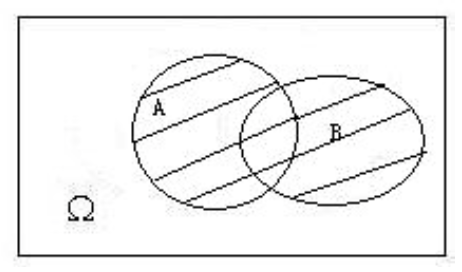
\includegraphics[width=3cm]{bing.png}

  \end{figure}}

  % \column{4cm}
  \pause
  \begin{exam}
    考虑掷一枚骰子, 观察出现的点数. 记事件$A$为掷出的点数为奇数, 事件$B$为掷出的点数不超过$3$, 则
    \[A=\{1,3,5\},\quad  B=\{1,2,3\},\quad  A\cup B=\{1,2,3,5\}\]

  \end{exam}


  % \end{columns}
\end{frame}
%\subsection{事件及其运算关系}

\begin{frame}
  \frametitle{事件间的交:$A\cap B$}
  % \begin{columns}
  %   \column{5cm}

  \begin{defi} (\tc{ 事件$A$与事件$B$的交}) 记为 $A\cap B$或 $AB$, 其含义为:事件$A$和事件$B$同时发生, 即由事件$A$与$B$中公共的样本点组成的新事件.\pause 用数学符号来描述即为:
    \begin{eqnarray*}
      A\cap B:=\{\omega\in \Omega: \omega\in A \mbox{ 且 } \omega\in B\}
    \end{eqnarray*}
  \end{defi}
  \vspace{-0.7cm}
  \only<2->{\begin{figure}[htbp]\nonumber
    \centering
    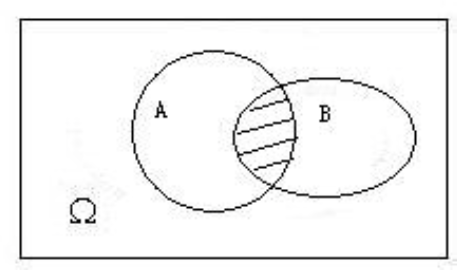
\includegraphics[width=3cm]{jiao.png}
  \end{figure}}

  % \column{4cm}
  \pause
  \begin{exam}
    考虑掷一枚骰子, 观察出现的点数. 记事件$A$为掷出的点数为奇数, 事件$B$为掷出的点数不超过$3$, 则
    \[A=\{1,3,5\},\quad  B=\{1,2,3\},\quad  A\cap B=\{1,3\}\]

  \end{exam}

\end{frame}


\begin{frame}
  \frametitle{事件的差:$A-B$}
  % \begin{columns}
  %   \column{5cm}

  \begin{defi} (\tc{ 事件$A$与$B$的差}) 记为$A-B$或$A\backslash B$, 其含义为:事件$A$发生且事件$B$不发生, 即由在$A$中而不在$B$中的样本点组成的新事件. \pause 用数学符号来描述即为:
    \begin{eqnarray*}
      A-B:=\{\omega\in \Omega: \omega\in  A \mbox{ 且 } \omega\notin B\}
    \end{eqnarray*}
  \end{defi}
  \vspace{-0.7cm}
  \only<2->{\begin{figure}[htbp]\nonumber

    \centering
    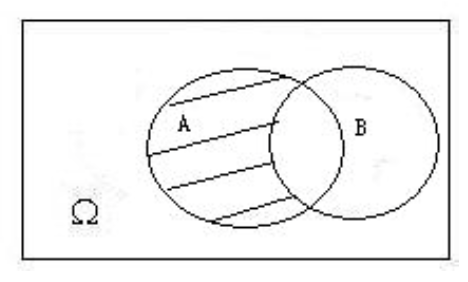
\includegraphics[width=3cm]{cha.png}

  \end{figure}}

  % \column{4cm}
  \pause
  \begin{exam}
    考虑掷一枚骰子, 观察出现的点数. 记事件$A$为掷出的点数为奇数, 事件$B$为掷出的点数不超过$3$, 则
    \[A=\{1,3,5\},\quad  B=\{1,2,3\},\quad  A-B=\{5\}\]   \end{exam}

\end{frame}


\begin{frame}
  \frametitle{对立事件:$\overline{A}$}
  % \begin{columns}
  %   \column{5cm}

  \begin{defi} (\tc{ 事件$A$的对立事件}) 记为$\overline{A}$或$A^c$, 其含义为:事件$A$不发生, 即由在$\Omega$中而不在$A$中的样本点组成的新事件.\pause 用数学符号来描述即为:
    \begin{eqnarray*}
      \overline{A}:=\{\omega\in \Omega: \omega\notin  A\}\textcolor{red}{=\Omega-A}
    \end{eqnarray*}
  \end{defi}
  \vspace{-0.7cm}
  \only<2->{ \begin{figure}[htbp]\nonumber

    \centering
    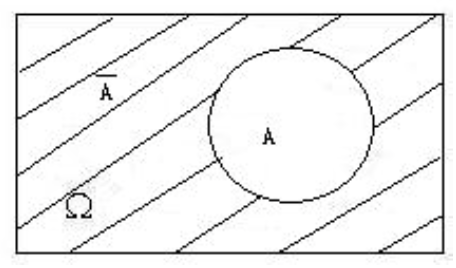
\includegraphics[width=3cm]{bu.png}

  \end{figure}}

  % \column{4cm}
  \pause
  \begin{exam}
    考虑掷一枚骰子, 观察出现的点数. 记事件$A$为掷出的点数为奇数, 则
    \[A=\{1,3,5\},\quad \overline{A}=\{2,4,6\}\]

  \end{exam}

\end{frame}
\begin{frame}
	\frametitle{对称差事件:$A\Delta B$}
	% \begin{columns}
		%   \column{5cm}

		\begin{defi} (\tc{ 事件$A$与$B$的对称差事件}) 记为$A\Delta B$, 其含义为:事件$A$与$B$中恰有一个事件发生.\pause 用数学符号来描述即为:
			\begin{eqnarray*}
				A\Delta B:=\{\omega\in \Omega: \omega\in A\cup B \mbox{ 且 } \omega\notin A\cap B\}\textcolor{red}{=(A-B)\cup (B-A)}
			\end{eqnarray*}
		\end{defi}
%		\vspace{-0.7cm}
%		\only<2->{ \begin{figure}[htbp]\nonumber
%
%				\centering
%				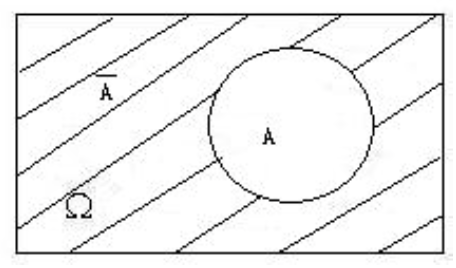
\includegraphics[width=3cm]{bu.png}
%
%		\end{figure}}
%
%		% \column{4cm}
%		\pause
%		\begin{exam}
%			考虑掷一枚骰子, 观察出现的点数. 记事件$A$为掷出的点数为奇数, 则
%			\[A=\{1,3,5\},\quad \overline{A}=\{2,4,6\}\]
%
%		\end{exam}

	\end{frame}


\begin{frame}
  \frametitle{包含关系: $A\subset B$}
  \begin{defi} (\tc{ 包含关系}) 称事件$A$包含于事件$B$,或事件$B$包含事件$A$(记为\tc{$A\subset B$}), 如果事件$A$发生必然导致事件$B$发生, 即属于$A$的样本点必然属于$B$.
  \end{defi}
  \pause
  \begin{exam}
    考虑掷一枚骰子, 观察出现的点数. 记事件$A$为掷出的点数为$2$或$4$, 事件$B$为掷出的点数为偶数. 则显然有事件$A$发生必然导致事件$B$发生,同时易知
    \begin{eqnarray*}
      A=\{2,4\}\subset \{2,4,6\}=B
    \end{eqnarray*}
  \end{exam}
\end{frame}

\begin{frame}
  \frametitle{相等关系: $A=B$}
  \begin{defi} (\tc{相等关系}) 称事件$A$与事件$B$相等(记为\tc{$A=B$}), 如果$A\subset B$且$B\subset A$, 即事情件$A,B$有相同的样本点.
  \end{defi}

  \pause
  \begin{exam}
    考虑掷一枚骰子, 观察出现的点数. 记事件$A$为掷出的点数为$2,4,6$, 事件$B$为掷出的点数为偶数. 则显然有
    \[A\subset B, B\subset A,\] 同时易有
    \begin{eqnarray*}
      A=\{2,4, 6\}=\{2,4,6\}=B
    \end{eqnarray*}

  \end{exam}
\end{frame}
\begin{frame}
  \frametitle{互不相容关系: $A\cap B=\emptyset$}
  \begin{defi} (\tc{ 互不相容关系}) 称事件$A$与事件$B$互不相容, 如果事件$A, B$不能同时发生, 即事情件$A,B$没有相同的样本点.
  \end{defi}

  \pause
  \vspace{1cm}
  \begin{exam}
    考虑掷一枚骰子, 观察出现的点数. 记事件$A$为掷出的点数为奇数, 事件$B$为掷出的点数为偶数. 则显然有事件$A,B$互不相容, 并且
    \begin{eqnarray*}
      A\cap B=\{1,3,5\}\cap \{2,4,6\}=\emptyset
    \end{eqnarray*}

  \end{exam}
\end{frame}

\begin{frame}
  \frametitle{对立事件与互不相容事件}
  \begin{itemize}[<+-|alert@+>]
  \item $\overline{\overline{A}}=A, A\cap \overline{A}=\emptyset, A\cup \overline{A}=\Omega$;
  \item $A,B$互为对立事件的充要条件为$A\cap B=\emptyset, A\cup B=\Omega$;
  \item 对立事件一定是互不相容事件, 但互不相容事件不一定是对立事件;
  \item $A-B=A\cap \overline{B}=A\overline{B}$
  \end{itemize}
\end{frame}

\begin{frame}{多个事件的运算}
	\begin{itemize}[<+-|alert@+>]

		\item 有限并事件:$\bigcup_{k=1}^{n}A_{k}$%:表示$n$个事件$A_1,A_2,...,A_n$至少有一个发生
		\item 有限交事件:$\bigcap_{k=1}^{n}A_{k}$%:表示$n$个事件$A_1,A_2,...,A_n$同时发生
		\item 可列并事件:$\bigcup_{k=1}^{\infty}A_{k}$%:$A_{1} \cup A_{2} \cup \cdots=\bigcup_{k=1}^{\infty} A_{k}=\lim _{n \rightarrow \infty} \bigcup_{k=1}^{n} A_{k}$
		\item 可列交事件:$\bigcap_{k=1}^{\infty}A_{k}$%:$A_{1} \cap A_{2} \cap \cdots=\bigcap_{k=1}^{\infty} A_{k}=\lim _{n \rightarrow \infty} \bigcap_{k=1}^{n} A_{k}$
		%\item 上极限事件$\bigcap_{k=1}^{\infty} \bigcup_{n=k}^{\infty} A_{n}$,其中$\left\{A_n,n\in\mathbb{Z}^+\right\}$是一列事件
		%\item 下极限事件$\bigcup_{k=1}^{\infty} \bigcap_{n=k}^{\infty} A_{n}$,其中$\left\{A_n,n\in\mathbb{Z}^+\right\}$是一列事件
	\end{itemize}
\end{frame}


\begin{frame}
	\frametitle{事件运算的性质}
	\begin{enumerate}[<+-|alert@+>][(1)]
		\item \tc{ 交换律:} $A\cup B=B\cup A, AB=BA$;
		\item \tc{ 结合律:} $A\cup (B\cup C)=(A\cup B)\cup C, (AB)C=A(BC)$;
		\item \tc{ 分配律:} $(A\cup B)\cap C=(A\cap C)\cup (B\cap C)$, \\\qquad \qquad $(A\cap B)\cup C=(A\cup C)\cap (B\cup C)$;
		\item \tc{{\rm De Morgan} 对偶法则:}
		\begin{eqnarray*}
			\overline{\bigcup_{i=1}^nA_i}=\bigcap_{i=1}^n \overline{A}_i\\
			\overline{\bigcap_{i=1}^nA_i}=\bigcup_{i=1}^n \overline{A}_i
		\end{eqnarray*}
	\end{enumerate}
\end{frame}


\subsection{事件列的上下极限及其性质}

\begin{frame}
	\frametitle{事件列的上下极限}
	\begin{defi}
		令$A_n\subset \Omega, n\geq 1$为一列集合(事件), 记
		\begin{eqnarray*}
			\inf_{k\geq n} A_k:=\cap_{k=n}^\infty A_k,\quad  \sup_{k\geq n}A_k:=\cup_{k=n}^\infty A_k
		\end{eqnarray*}
		则事件列$A_n$的上下极限定义如下:
		\begin{eqnarray*}
			\liminf_{n\rightarrow\infty}A_n:=\cup_{n=1}^\infty\cap_{k=n}^\infty A_k,\\%=\lim_{n\rightarrow\infty}\bigg(\inf_{k\geq n}A_k\bigg)\\
			\limsup_{n\rightarrow\infty}A_n:=\cap_{n=1}^\infty\cup_{k=n}^\infty A_k.
		\end{eqnarray*}
		若
		\begin{eqnarray*}
			\liminf_{n\rightarrow\infty}A_n=\limsup_{n\rightarrow\infty}A_n=A
		\end{eqnarray*}
		则称$A$为事件列$\{A_n,n\geq 1\}$的极限,并记作$\lim_{n\rightarrow\infty}A_n=A$.
	\end{defi}

\end{frame}


\begin{frame}
	\frametitle{单调事件列的极限}
	\begin{defi}
		事件列$\{A_n\}$称为单调不减的,如果对任意的$n$均有$A_n\subset A_{n+1}$;     事件列$\{A_n\}$称为单调不增的,如果对任意的$n$均有$A_{n+1}\subset A_n$;
	\end{defi}
	\vspace{0.4cm}

	\pause


	\begin{thm}
		假设$\{A_n\}$是单调事件列,则
		\begin{enumerate}
			\item 如果$\{A_n\}$是单调不减事件列,则$\lim_{n\rightarrow\infty}A_n=\cup_{n=1}^\infty A_n$
			\item 如果$\{A_n\}$是单调不增事件列,则$\lim_{n\rightarrow\infty}A_n=\cap_{n=1}^\infty A_n$
		\end{enumerate}

	\end{thm}

\end{frame}


\begin{frame}
	\frametitle{示性函数({\rm indicator function})}
	\begin{defi}
		设$A\subset \Omega$, 我们定义事件(集合)$A$的示性函数如下
		\begin{eqnarray*}
			1_A(\omega)=\left\{
			\begin{array}[l]{ll}
				1, &\mbox{如果}\omega\in A;\\
				0, &\mbox{如果}\omega\notin A.
			\end{array}
			\right.
		\end{eqnarray*}

	\end{defi}

	\begin{rmk}
		\begin{itemize}[<+-|alert@+>]

			\item $A=\{\omega: 1_A(\omega)=1\}$;
			\item $1_A\leq 1_B\Leftrightarrow A\subset B$;
			\item $1_{A\cap B}=1_A\cdot 1_B$;
			\item $1_{A\cup B}=1_A+1_B-1_{A\cap B}$;
		\end{itemize}
	\end{rmk}
\end{frame}

\begin{frame}
	\frametitle{事件列上下极限的性质}
	\begin{lem}
		令$\{A_n\}$为$\Omega$的任一子集列,则
		\begin{eqnarray*}
			\limsup_{n\rightarrow\infty}A_n&=&\{\omega:\sum_{n=1}^\infty 1_{A_n}(\omega)=\infty\}\\
			&=&\{\omega: \omega\mbox{属于无穷多个}A_n\}\\
			\liminf_{n\rightarrow\infty}A_n&=&\{\omega:\sum_{n=1}^\infty 1_{\bar{A_n}}(\omega)<\infty\}\\
			&=&\{\omega:\mbox{除去有限多个}A_n\mbox{外},\omega\mbox{属于余下所有的}A_n\}
		\end{eqnarray*}
	\end{lem}\pause
	\zheng 由$\omega\in \limsup_{n\rightarrow\infty}A_n=\cap_{n=1}^\infty \cup_{k=n}^\infty A_k$知,对任意的$n$, 存在 $k_n\geq n$使得$\omega\in A_{k_n}$, 从而$\sum_{n=1}^\infty 1_{A_n}\geq \sum_{n=1}^\infty 1_{A_{k_n}}=\infty $.\pause

	\qquad 反之,若 $\omega\in \{\omega:\sum_{n=1}^\infty 1_{A_n}(\omega)=\infty\}$, 则存在$k_n\rightarrow\infty$使得$\omega\in A_{k_n}$, 从而对任意的$n$, $\omega\in\cup_{k=n}^\infty A_k$, 即 $$\omega\in \cap_{n=1}^\infty \cup_{k=n}^\infty A_k=\limsup_{n\rightarrow\infty} A_n.$$
\end{frame}


\subsection{事件运算表及例子}

\begin{frame}
	\frametitle{事件运算表}
	% \begin{columns}
		%   \column{5cm}

	\begin{figure}[htbp]\nonumber

				\centering
				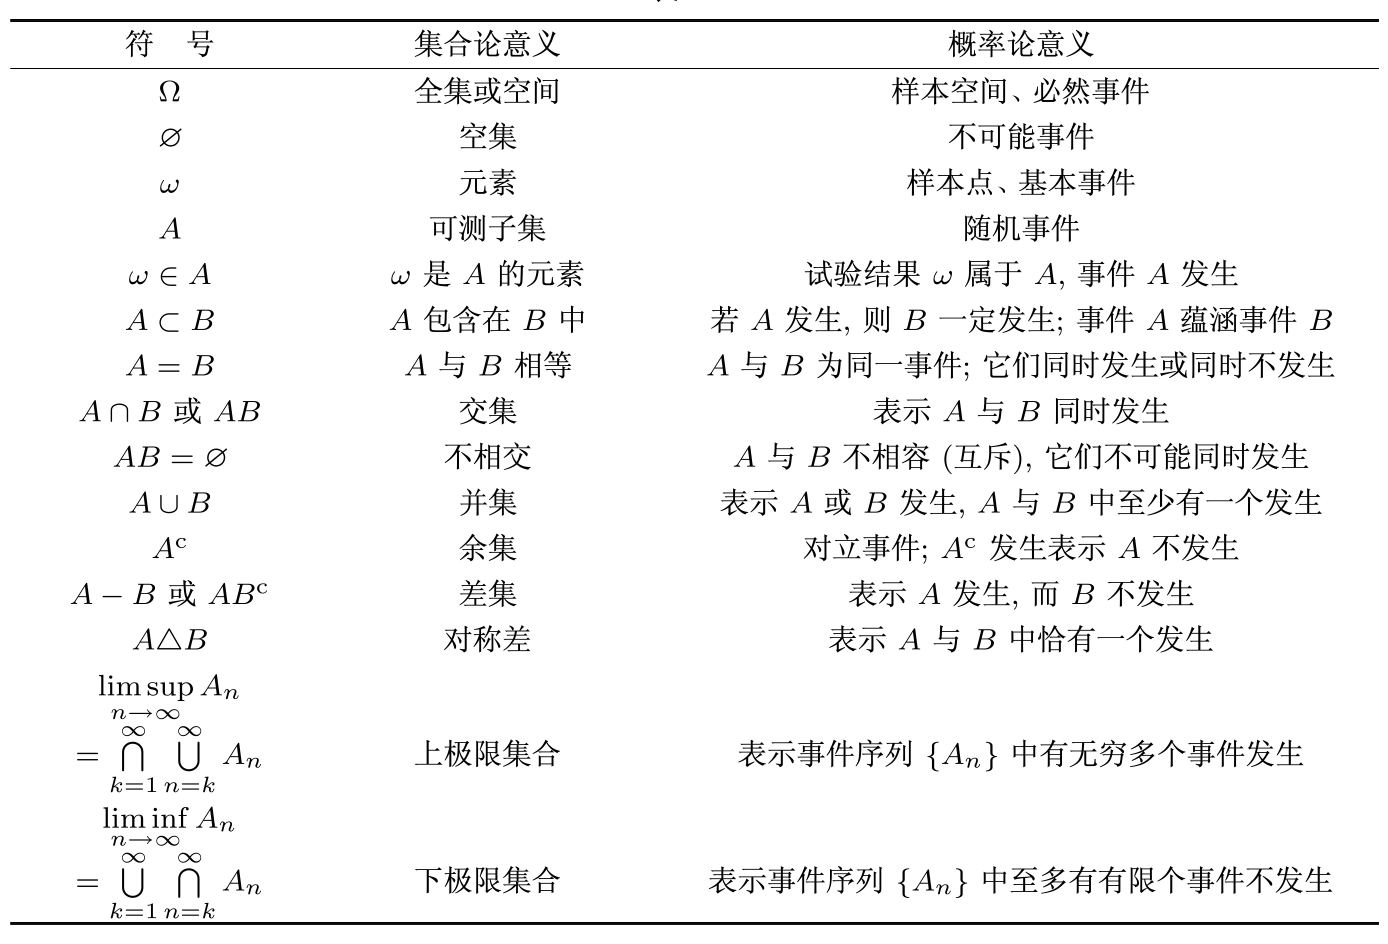
\includegraphics[width=12cm,height=7cm]{eventable.png}

		\end{figure}

	\vspace{1cm}
	\end{frame}










\begin{frame}
  \begin{exam}
    设$A,B,C$为某个随机现象的三个事件,试用事件的交,差,并,对立事件表示下列事件
    \begin{itemize}[<+-|alert@+>]
    \item 事件$A,B$发生而$C$不发生:\pause\textcolor{red}{$AB\overline{C}$};
    \item 事件$A,B,C$中至少有一个发生:\pause \trc{$A\cup B\cup C$};
    \item 事件$A,B,C$中至少有两个发生:\pause \trc{ $AB\cup AC\cup BC$};
    \item 事件$A,B, C$中恰好有两个发生:\pause \trc{ $AB\overline{C}\cup A\overline{B}C\cup \overline{A}BC$};
    \item 事件$A,B,C$同时发生:\pause \trc{ $ABC$};
    \item 事件$A,B,C$都不发生:\pause \trc{ $\overline{A}\cap \overline{B}\cap  \overline{C}$};
    \item 事件$A,B,C$不全发生:\pause \trc{ $\overline{A}\cup \overline{B}\cup  \overline{C}$};
    \end{itemize}

  \end{exam}
\end{frame}

\begin{frame}
	 \begin{exam} (掷硬币) 掷一枚硬币$10$次, 正面用${\mathrm{H}}$表示反面用${\mathrm{T}}$表示.
	 	    \begin{itemize}[<+-|alert@+>]
	 	    	\item 一个可能的结果为{\rm HHHTHHTTHT}, \pause 且样本空间就是所有长度为$10$的由${\mathrm{H}}$和${\mathrm{T}}$组成的字符串的集合
	 	    	\item 若令${\mathrm{H}}$为$1$,${\mathrm{T}}$为$0$ , 则一个结果可用数列${\left(s_{1}, s_{2}, \cdots, s_{10}\right)}$表示, 其中${s_{j} \in\{0,1\}}$, 样本空间即为这些数列的集合
	 	    	\item 下面我们看几个事件:
   		 	    \begin{itemize}[<+-|alert@+>]
	\item ${A_{i}}$: 第$i$次掷硬币结果为${\mathrm{H}}$,则\pause
	\[
	A_{1}=\left\{\left(1, s_{2}, \cdots, s_{10}\right): s_{j} \in\{1,0\} \text{ 且 } 2 \leqslant j \leqslant 10\right\}.
	\]
	\item %这是样本空间的一个子集, 所以可以将它看作一个事件; 事件 ${A_{1}}$ 发生等价于第一次掷
	${B}$: 至少有一次掷硬币结果为${\mathrm{H}}$, 则\pause $B=\bigcup_{j=1}^{10} A_{j}.$
	\item ${C}$: 所有掷硬币结果都为${\mathrm{H}}$, 则\pause $C=\bigcap_{j=1}^{10} A_{j}.$
	\item ${D}$: 至少有两个连续的${\mathrm{H}}$,  则\pause $D=\bigcup_{j=1}^{9}\left(A_{j} \cap A_{j+1}\right).$
	    \end{itemize}
    	    \end{itemize}
	  \end{exam}
\end{frame}
